\chapter{HASIL DAN PEMBAHASAN}
\label{chap:hasilpembahasan}

% Ubah bagian-bagian berikut dengan isi dari hasil dan pembahasan

Bab ini akan membahas hasil dan analisa dari desain sistem yang sudah dibuat dan implementasinya. Pengujian terhadap hasil dibagi menjadi beberap bagian.

\section{Pengujian Performa antar \emph{Weight}}

\subsection{Pengujian Performa \emph{Weight} Hasil \emph{Pretrain} COCO Dataset}


\begin{longtable}{|c|c|c|c|c|}
  \caption{Konfigurasi Training menggunakan YOLOv5}
  \label{tb:pretraincoco}\\
  \hline
  \rowcolor[HTML]{C0C0C0}
  \textbf{\emph{Pretrained Weight}} & \emph{Precision}  & \emph{Recall} & \emph{mAP@.5} & \emph{Inference Time}\\
  \hline
  YOLOv5n                           & 0.92              & 0.878         & 0.922         & 1.9ms                \\
  YOLOv5s                           & 0.927              & 0.882         & 0.929         & 4.1ms             \\
  YOLOv5m                           & 0.923             & 0.892         & 0.933        & 9ms                \\
  YOLOv5l                           & 0.917            & 0.87         & 0.919         & 13.9ms                \\
  \hline
\end{longtable}

\subsection{Pengujian Performa \emph{Weight} Hasil Train Murni Dataset Deteksi Helm Keselamatan Kerja}

\begin{longtable}{|c|c|c|c|c|}
  \caption{Konfigurasi Training menggunakan YOLOv5}
  \label{tb:nopretrain}\\
  \hline
  \rowcolor[HTML]{C0C0C0}
  \textbf{\emph{Pretrained Weight}} & \emph{Precision}  & \emph{Recall} & \emph{mAP@.5} & \emph{Inference Time}\\
  \hline
  YOLOv5n                           & 0.918              & 0.85         & 0.909         & 2.4ms                \\
  YOLOv5s                           & 0.927             & 0.865        & 0.919        & 4.1ms               \\
  YOLOv5m                           & 0.939            & 0.862        & 0.924        & 8.7ms                \\
  YOLOv5l                           &                   &             &               &                \\
  \hline
\end{longtable}

\section{Pengujian Performa Berdasarkan Jarak}

\subsection{Pengujian Pada Jarak 1.3 Meter}

\begin{figure}[ht]
  \centering
  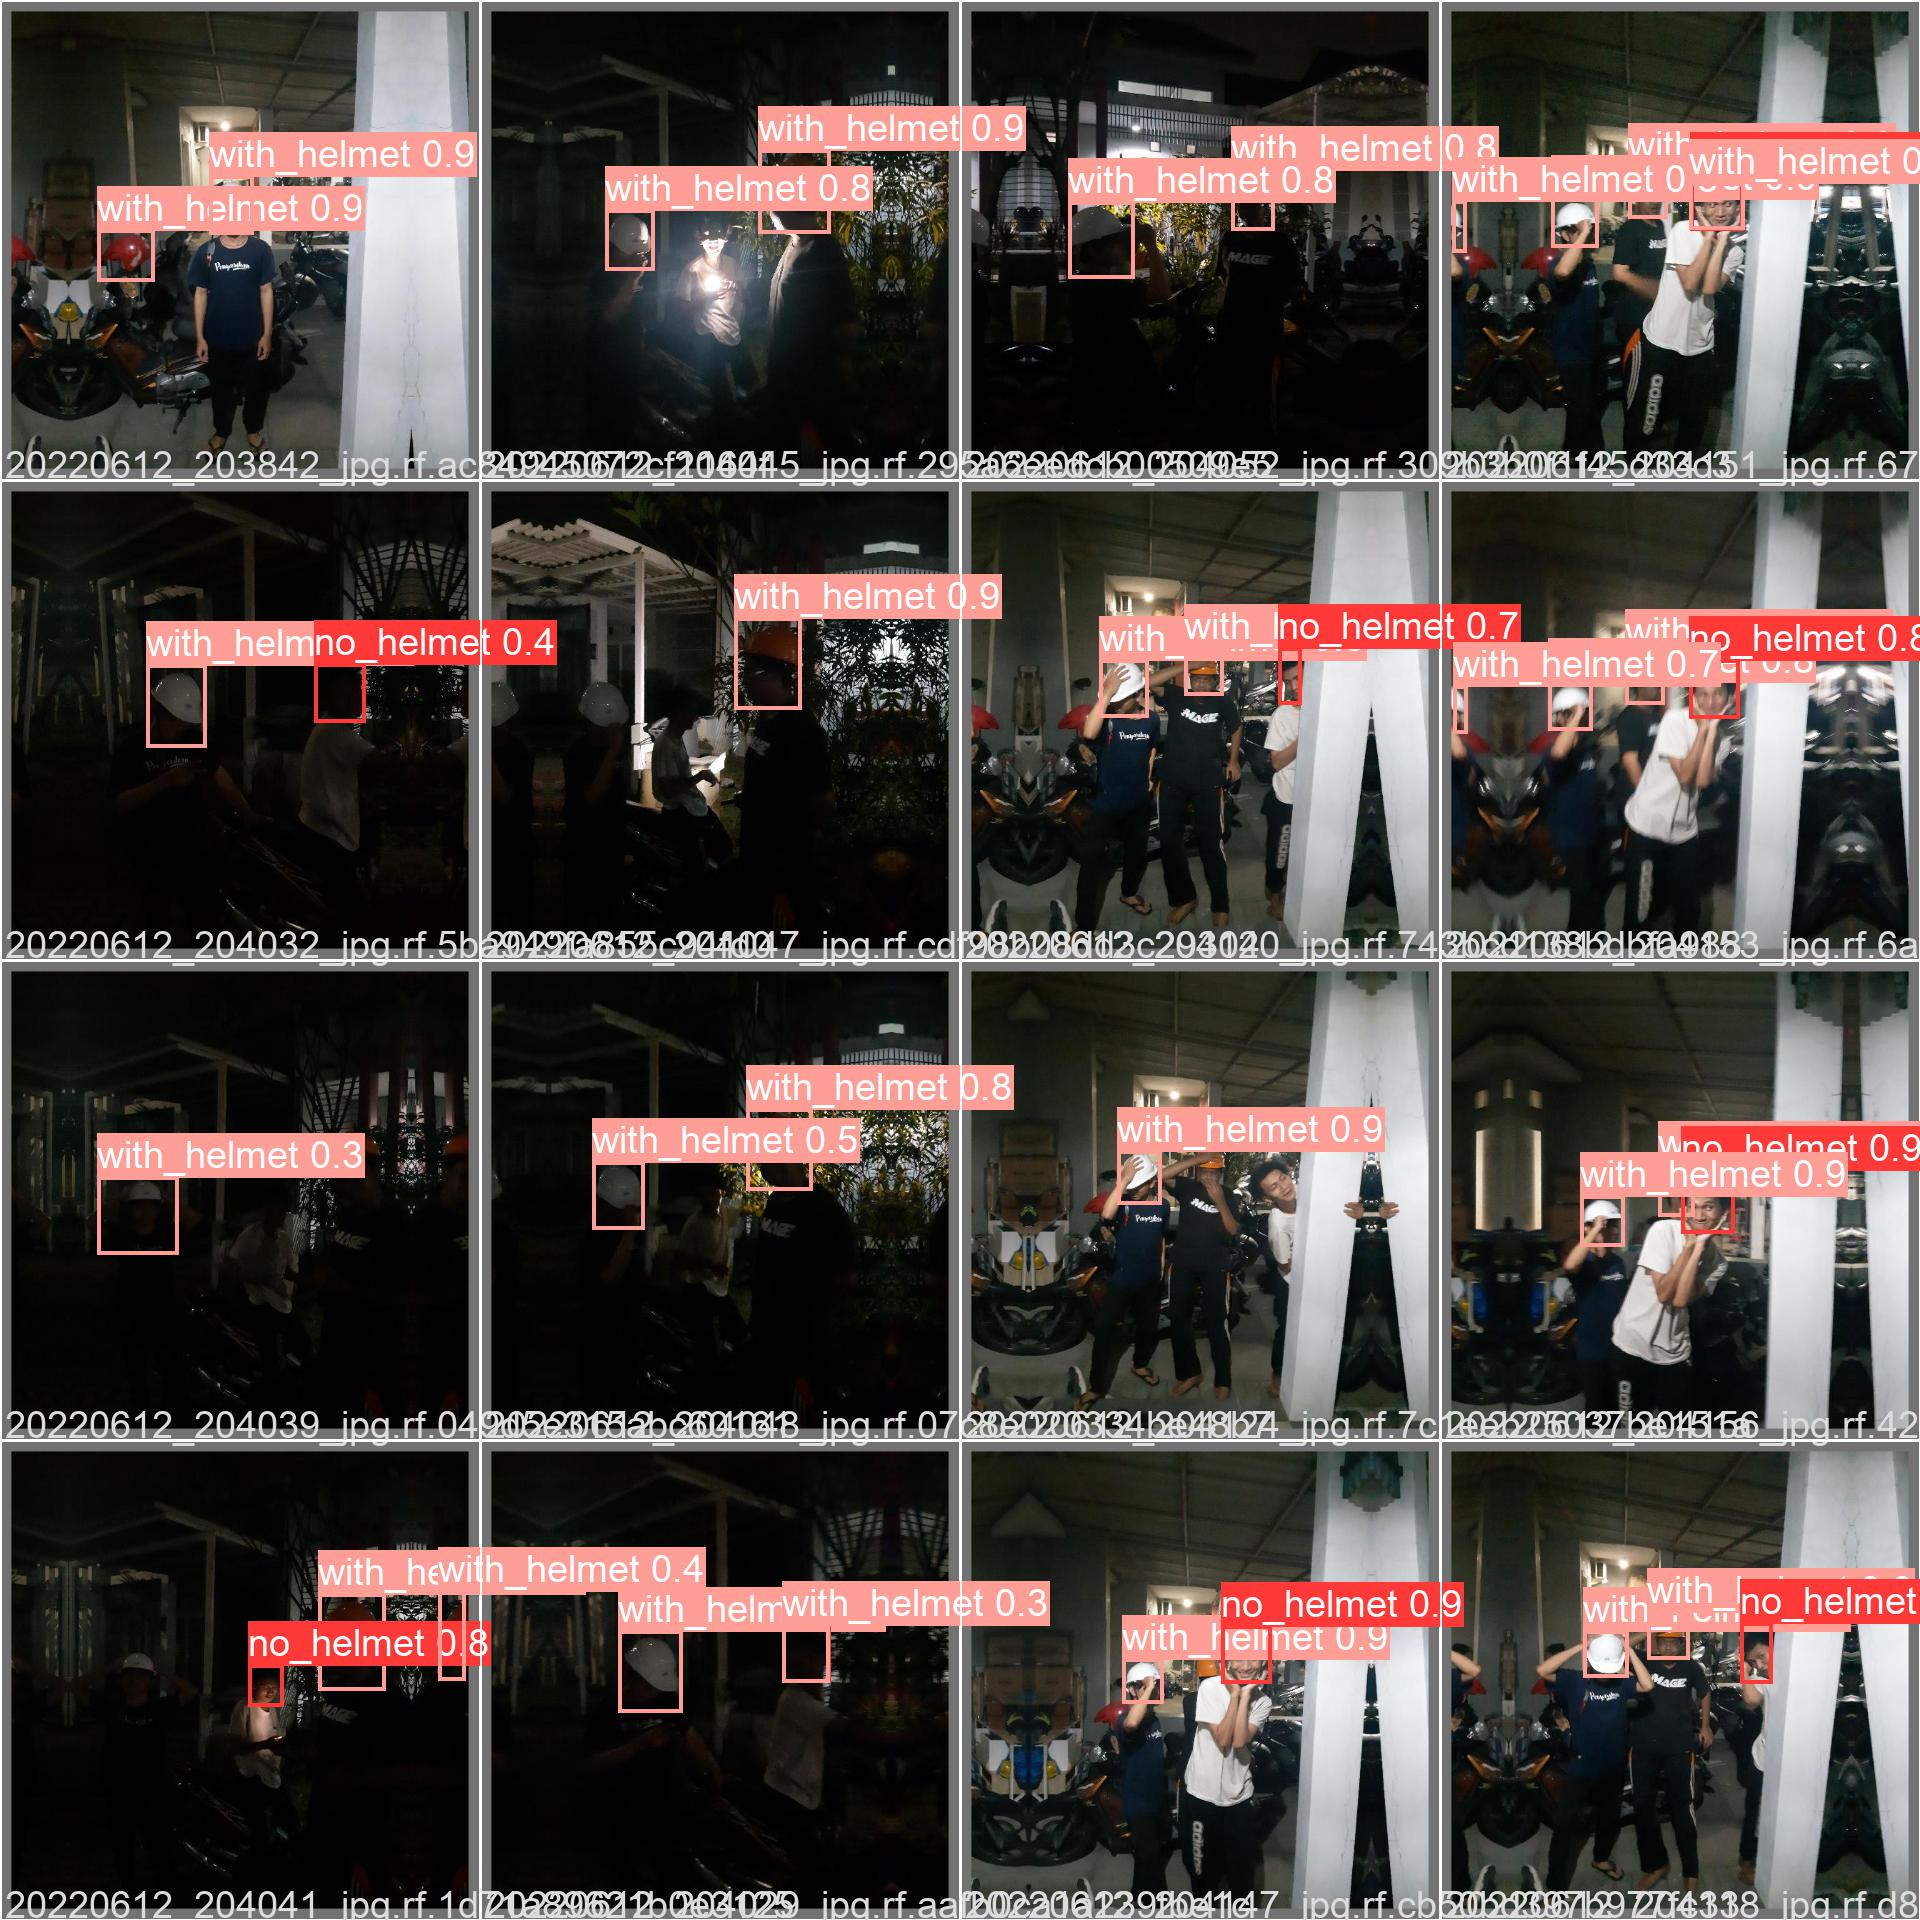
\includegraphics[scale=0.1]{gambar/BerdasarkanJarak/Jarak1.3/val_batch0_pred.jpg}
  \caption{Hasil Prediksi Pada Jarak 1.3 meter}
  % \label{fig:labelbaru}  
\end{figure}

\begin{longtable}{|c|c|c|c|}
  \caption{Konfigurasi Training menggunakan YOLOv5}
  \label{tb:wkwkw}\\
  \hline
  % \rowcolor[HTML]{C0C0C0}
  \textbf{\emph{Class} }                     & \textbf{\emph{Precision}}  & \textbf{\emph{Recall}} & \textbf{\emph{mAP@.5}}\\
  \hline
  all                                                 & 0.998           & 0.8     & 0.995         \\
  no\textunderscore helmet                            & 1               & 0.6       & 0.995          \\
  with\textunderscore helmet                          & 0.996           & 1       & 0.995            \\
  \hline
\end{longtable}

\subsection{Pengujian Pada Jarak 2.6 Meter}

\begin{figure}[ht]
  \centering
  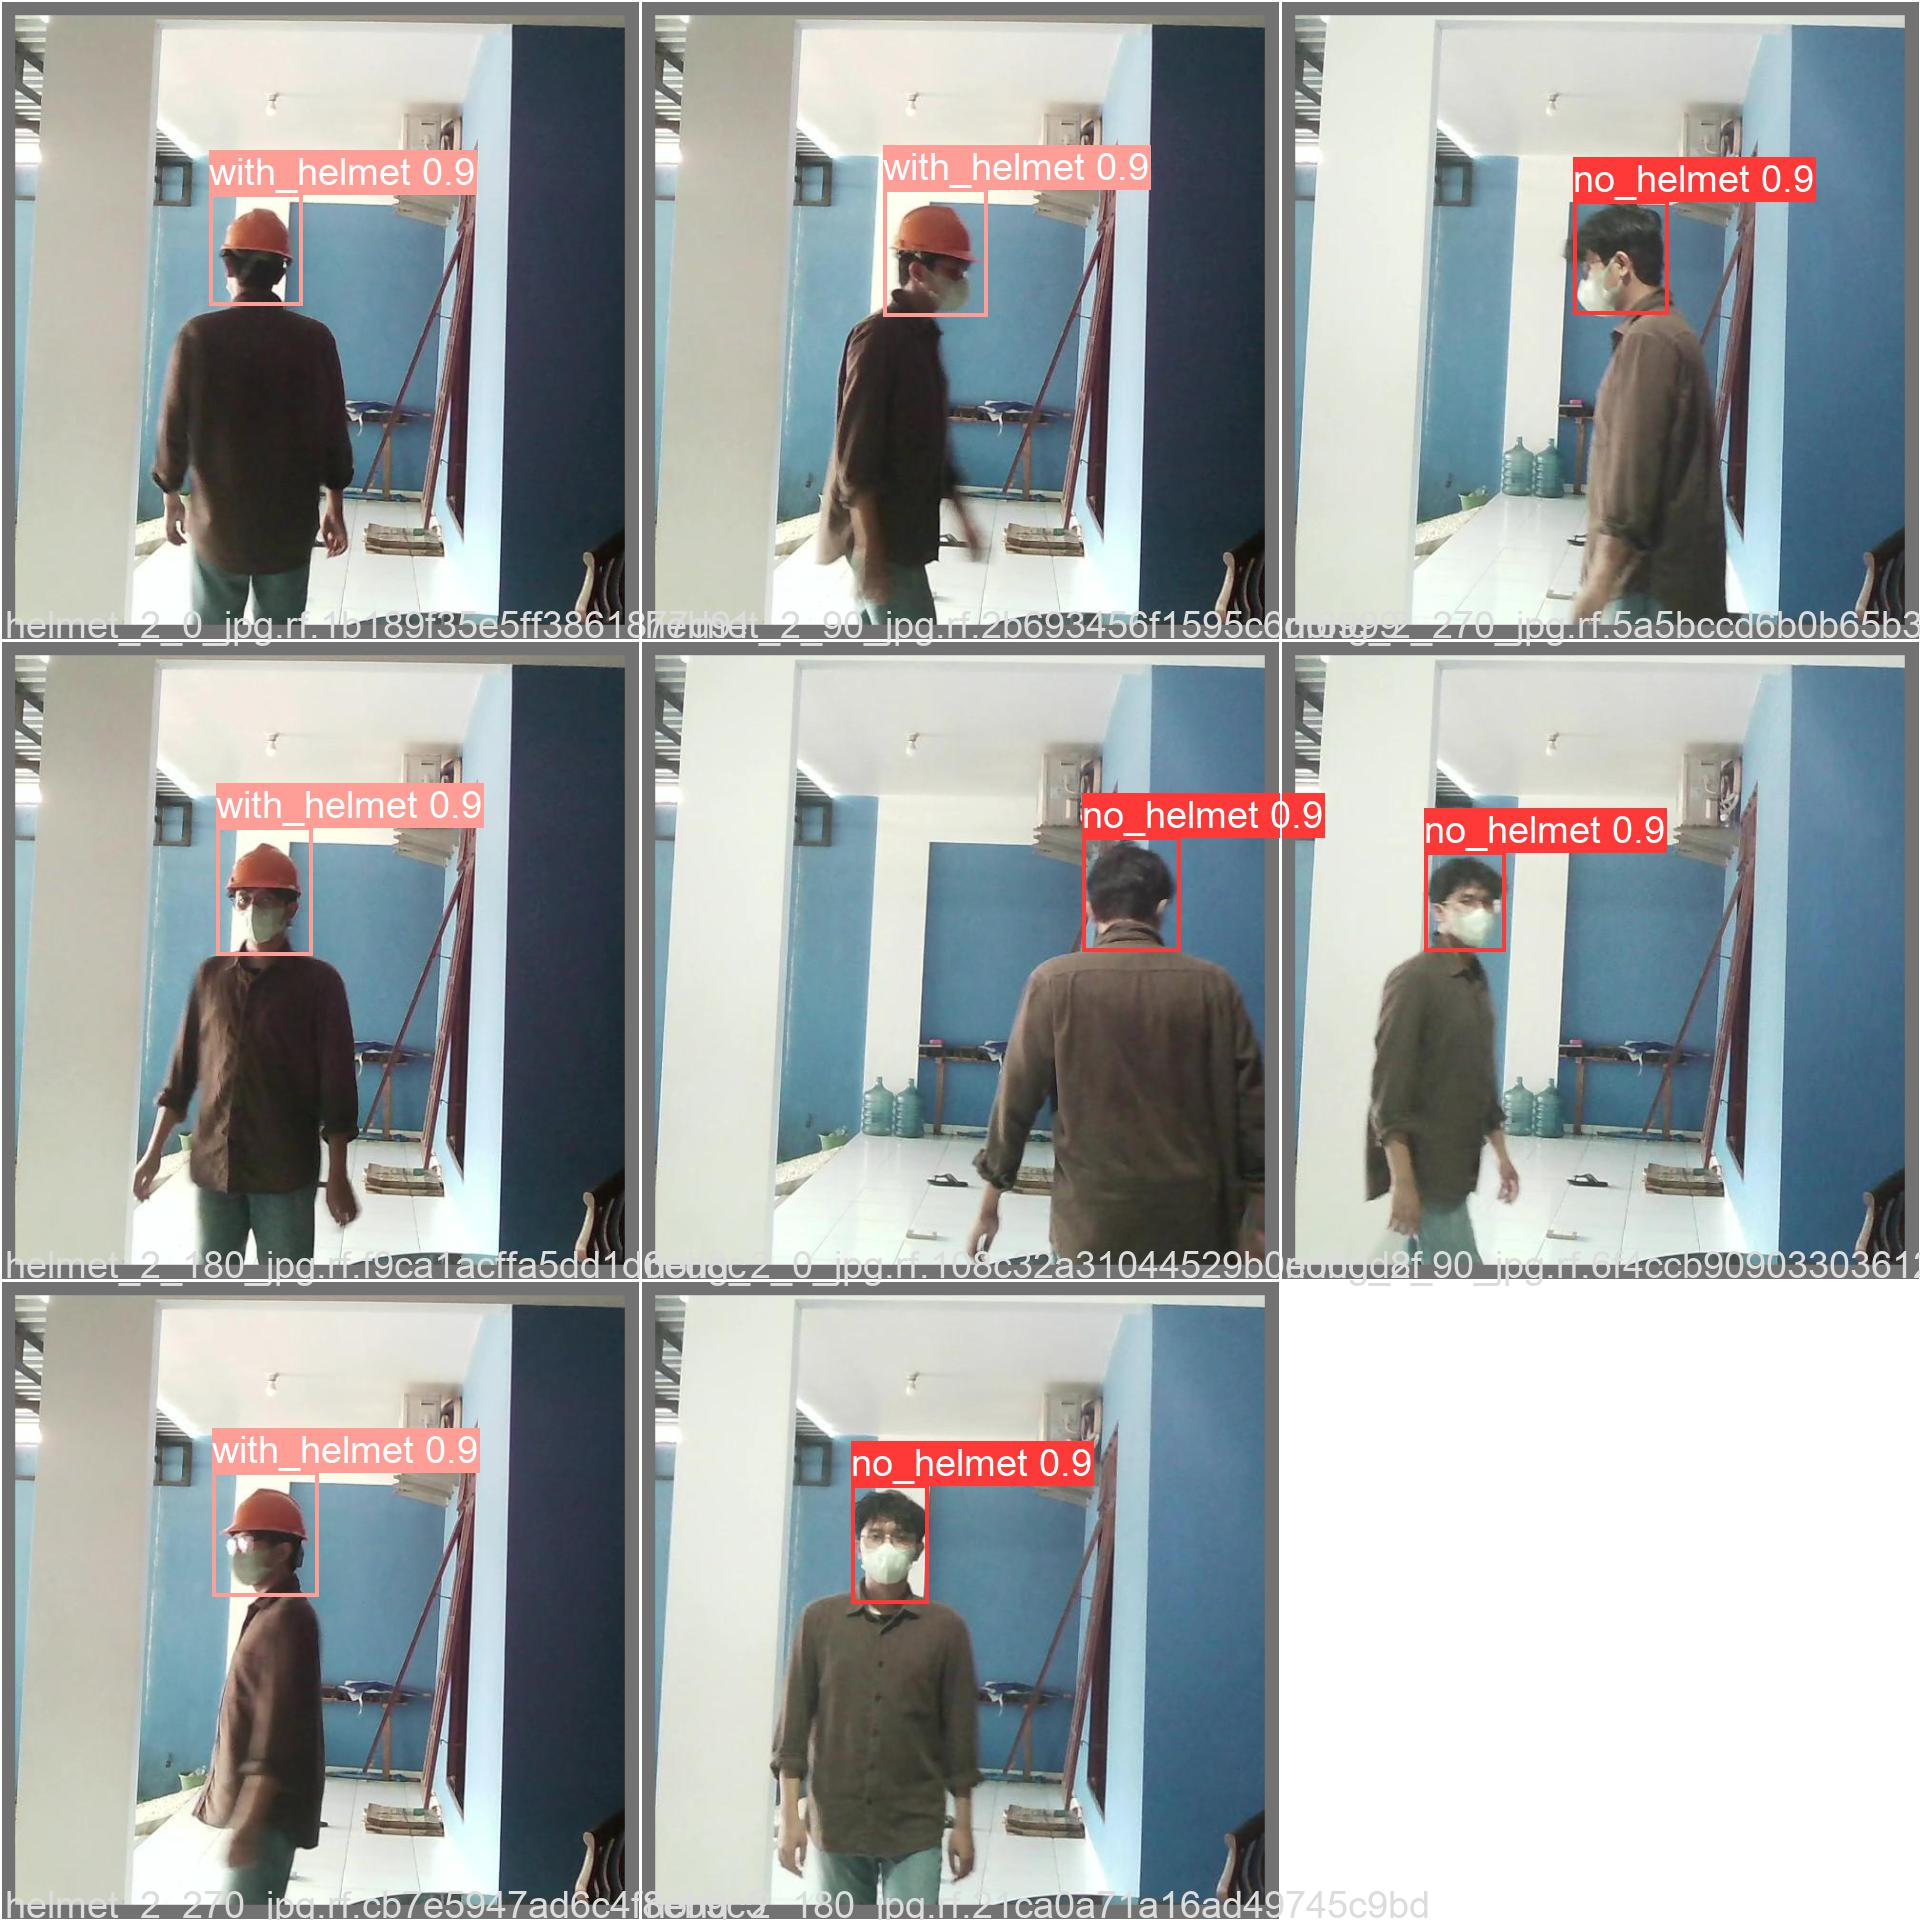
\includegraphics[scale=0.1]{gambar/BerdasarkanJarak/Jarak2_6/val_batch0_pred.jpg}
  \caption{Hasil Prediksi Pada Jarak 2.6 meter}
  % \label{fig:labelbaru}  
\end{figure}

\begin{longtable}{|c|c|c|c|}
  \caption{Konfigurasi Training menggunakan YOLOv5}
  \label{tb:jarak2_6}\\
  \hline
  % \rowcolor[HTML]{C0C0C0}
  \textbf{\emph{Class} }                     & \textbf{\emph{Precision}}  & \textbf{\emph{Recall}} & \textbf{\emph{mAP@.5}}\\
  \hline
  all                                                 & 0.996            & 1        & 0.995         \\
  no\textunderscore helmet                            & 1                & 1        & 0.995          \\
  with\textunderscore helmet                          & 0.992            & 1        & 0.995           \\
  \hline
\end{longtable}

\subsection{Pengujian Pada Jarak 4 Meter}

\begin{figure}[t]
  \centering
  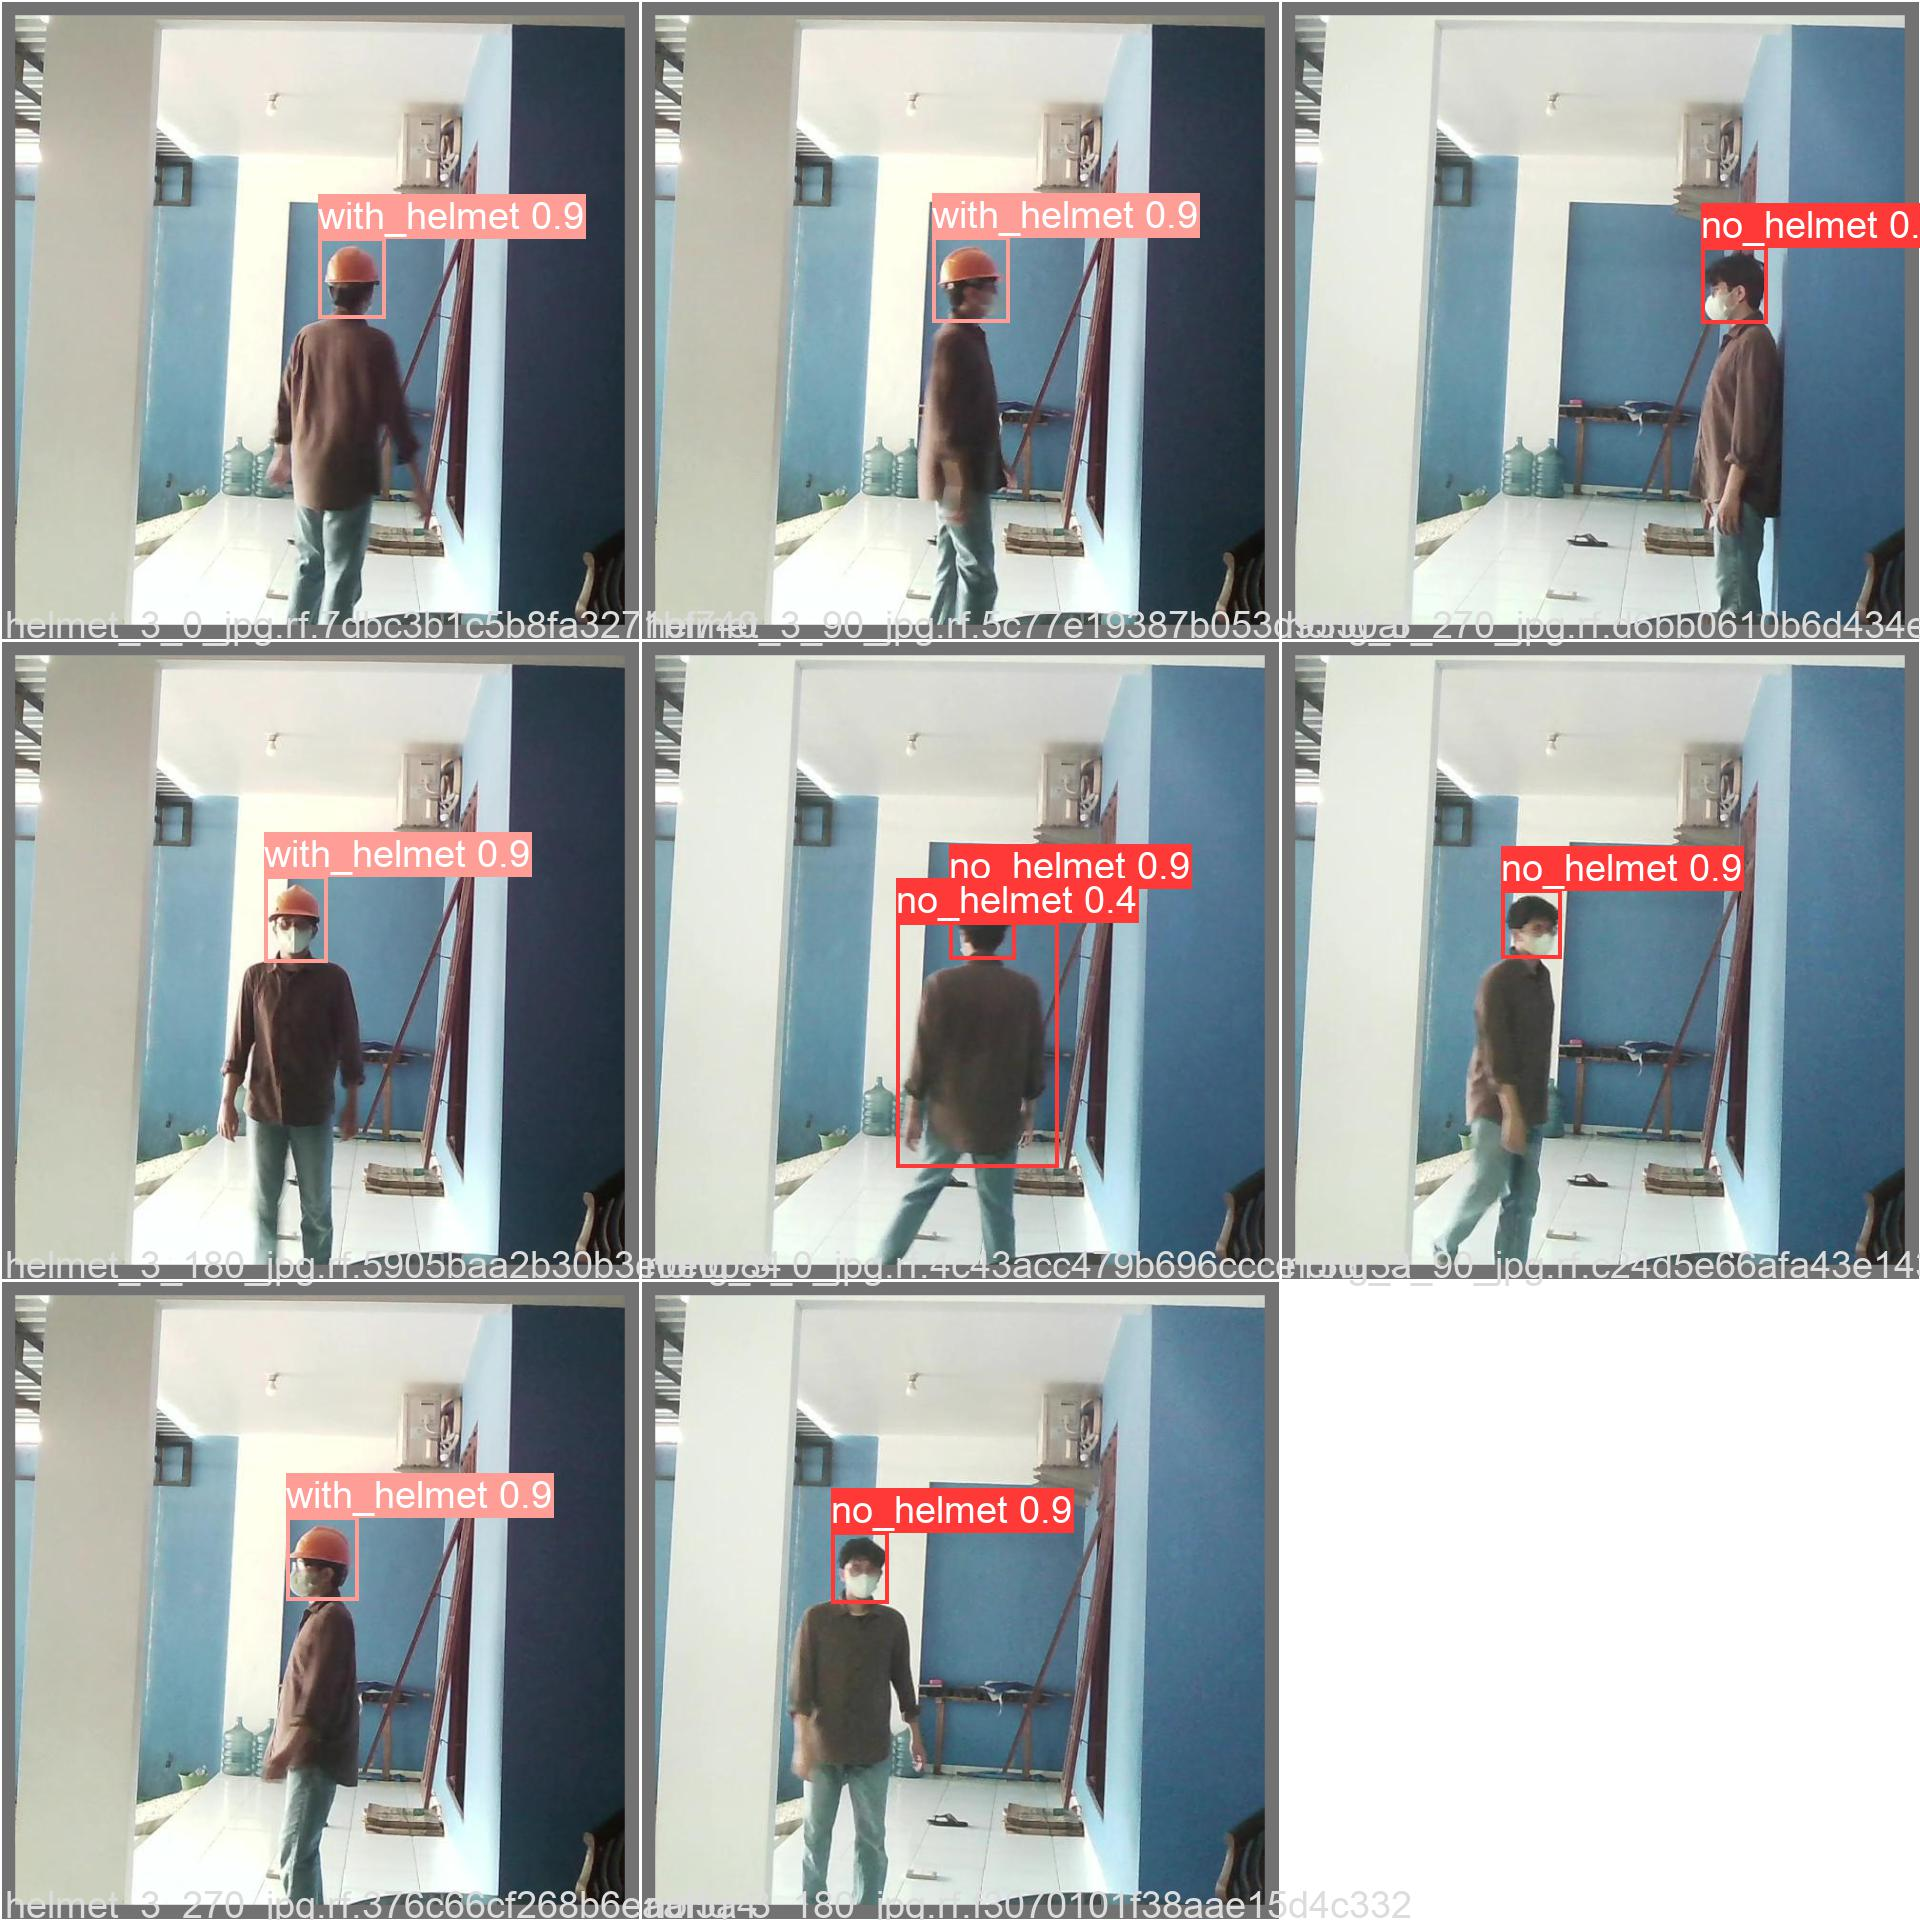
\includegraphics[scale=0.1]{gambar/BerdasarkanJarak/Jarak4/val_batch0_pred.jpg}
  \caption{Hasil Prediksi Pada Jarak 4 meter}
  % \label{fig:labelbaru}  
\end{figure}

\begin{longtable}{|c|c|c|c|}
  \caption{Konfigurasi Training menggunakan YOLOv5}
  \label{tb:jarak4}\\
  \hline
  % \rowcolor[HTML]{C0C0C0}
  \textbf{\emph{Class} }                     & \textbf{\emph{Precision}}  & \textbf{\emph{Recall}} & \textbf{\emph{mAP@.5}}\\
  \hline
  all                                                 & 0.981           & 1        & 0.995         \\
  no\textunderscore helmet                            & 1               & 1        & 0.995          \\
  with\textunderscore helmet                          & 0.963           & 1        & 0.995           \\
  \hline
\end{longtable}

\subsection{Pengujian Pada Jarak 5.3 Meter}

\begin{figure}[ht]
  \centering
  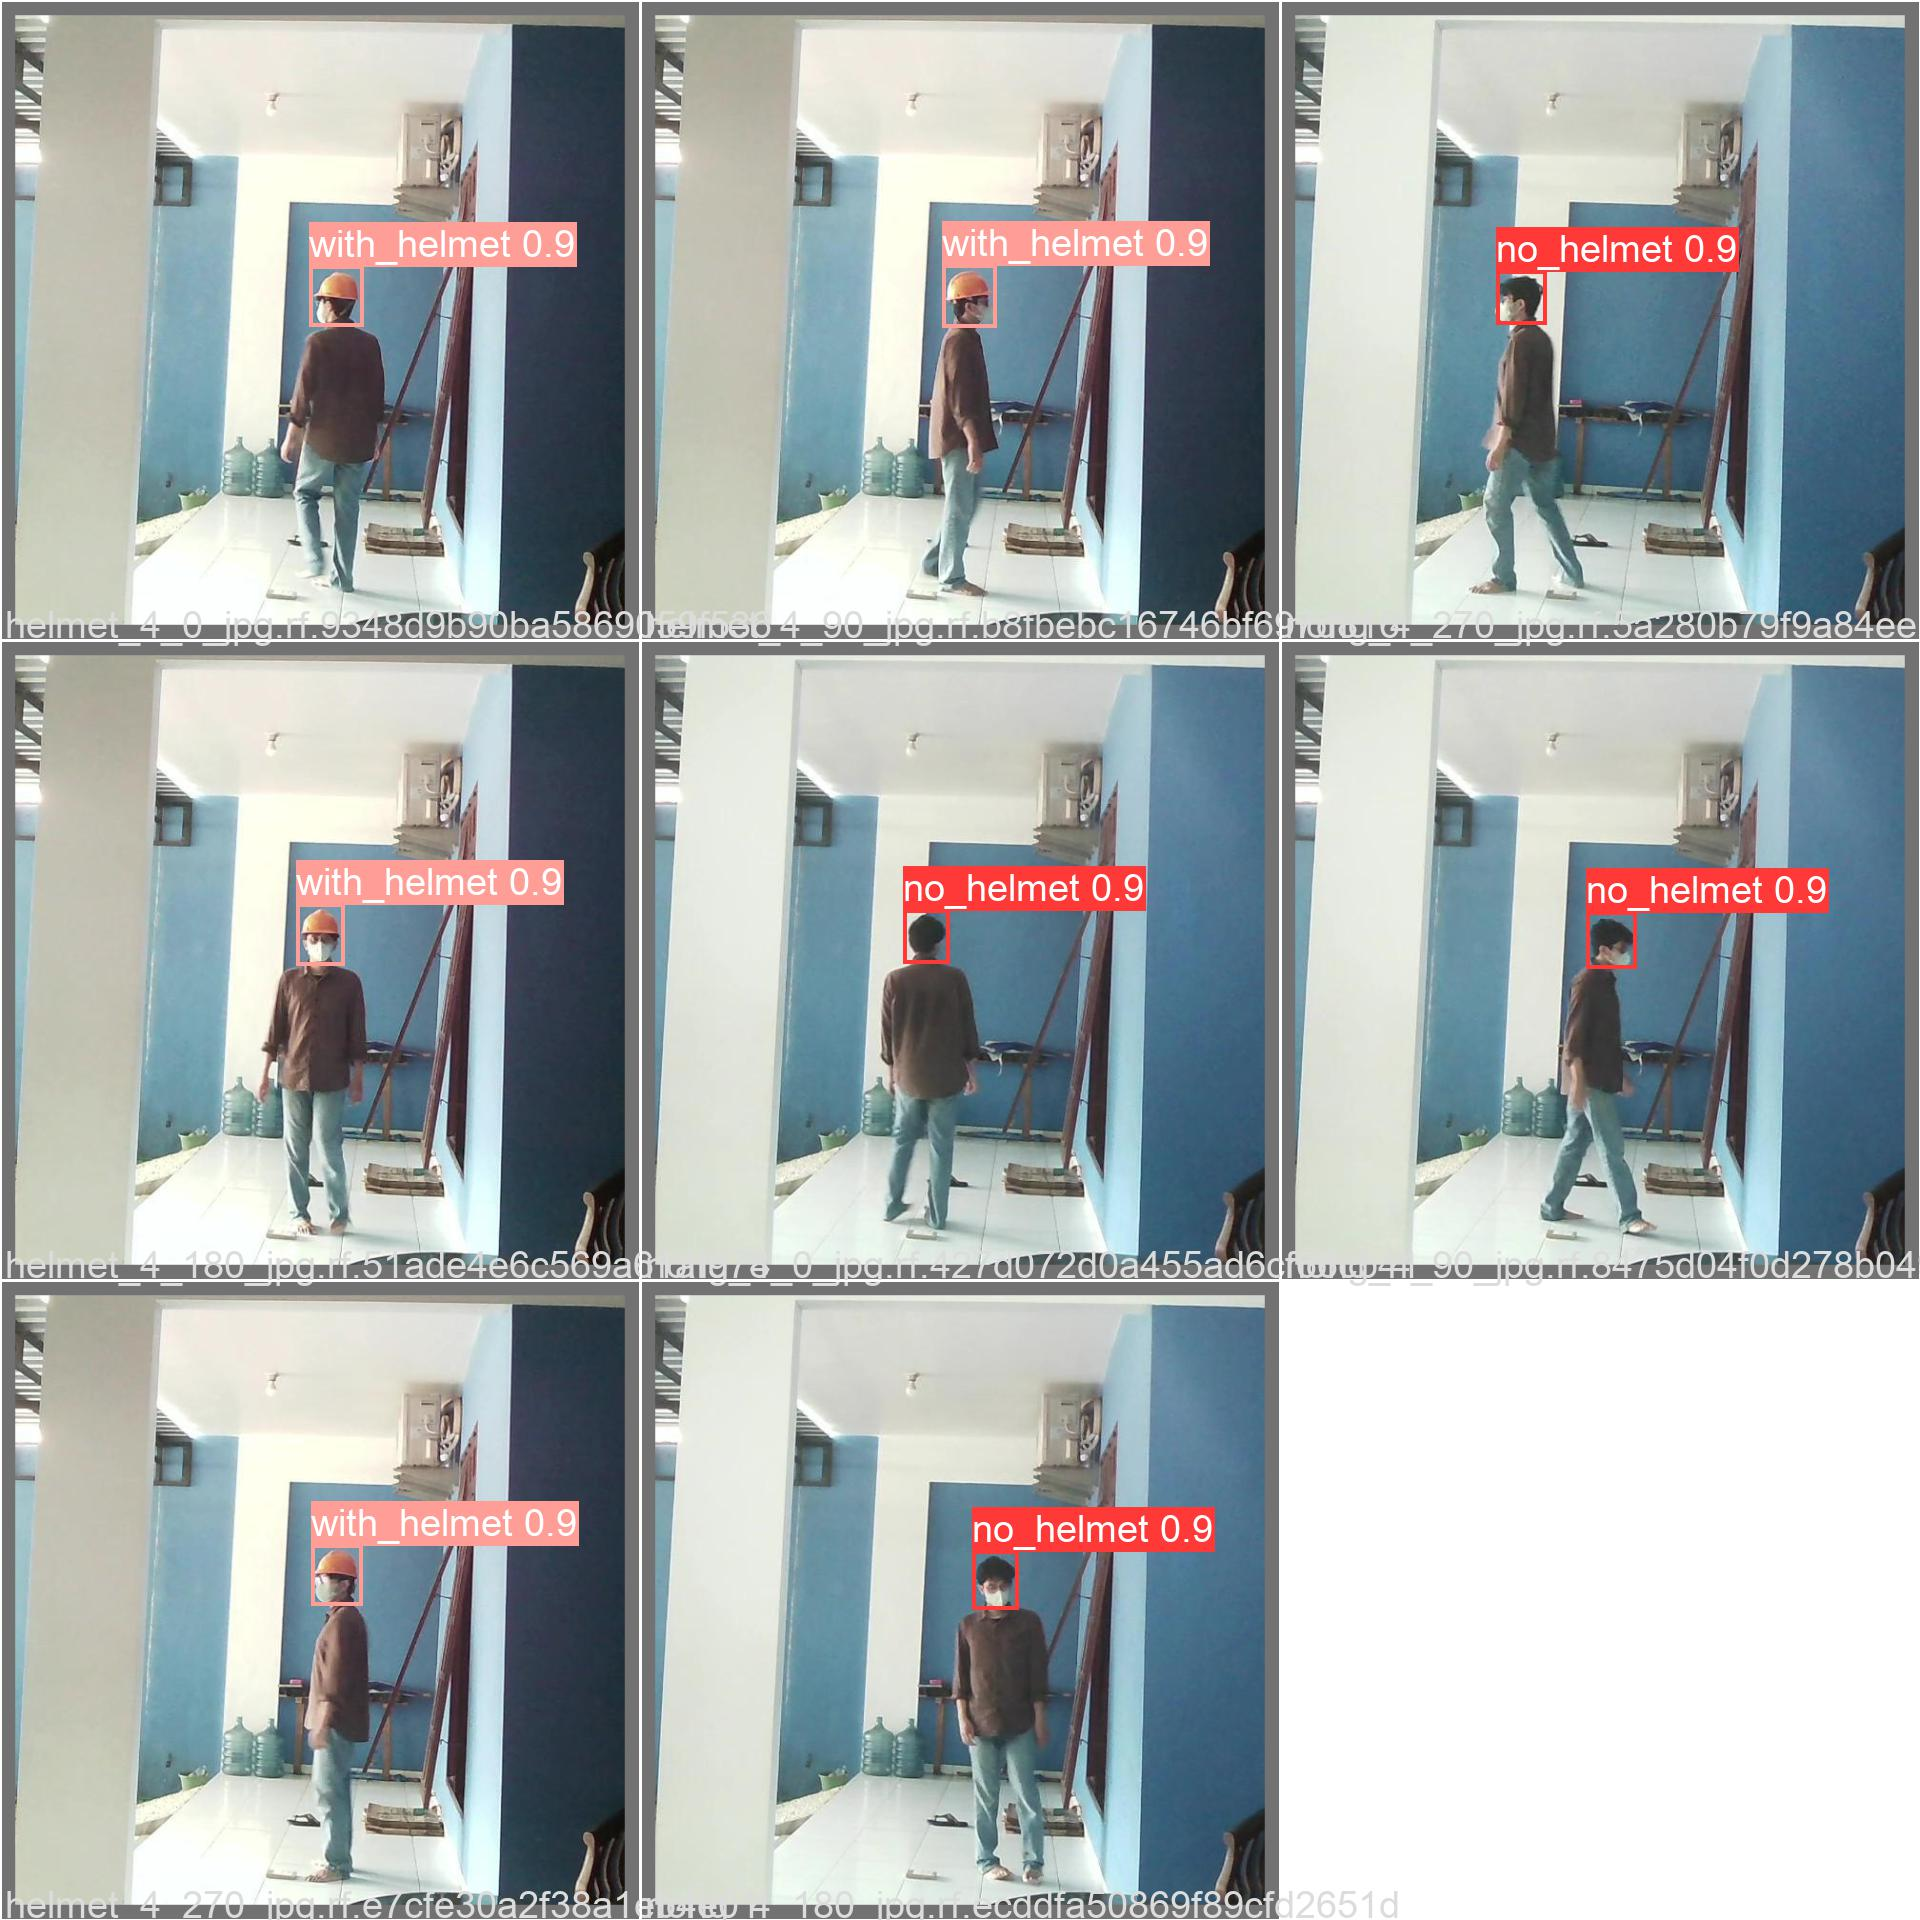
\includegraphics[scale=0.1]{gambar/BerdasarkanJarak/Jarak5_3/val_batch0_pred.jpg}
  \caption{Hasil Prediksi Pada Jarak 5.3 meter}
  % \label{fig:labelbaru}  
\end{figure}

\begin{longtable}{|c|c|c|c|}
  \caption{Konfigurasi Training menggunakan YOLOv5}
  \label{tb:jarak5_3}\\
  \hline
  % \rowcolor[HTML]{C0C0C0}
  \textbf{\emph{Class} }                     & \textbf{\emph{Precision}}  & \textbf{\emph{Recall}} & \textbf{\emph{mAP@.5}}\\
  \hline
  all                                                 & 0.997           & 1        & 0.995         \\
  no\textunderscore helmet                            & 1               & 1        & 0.995          \\
  with\textunderscore helmet                          & 0.995           & 1        & 0.995           \\
  \hline
\end{longtable}

\subsection{Pengujian Pada Jarak 6.7 Meter}

\begin{figure}[ht]
  \centering
  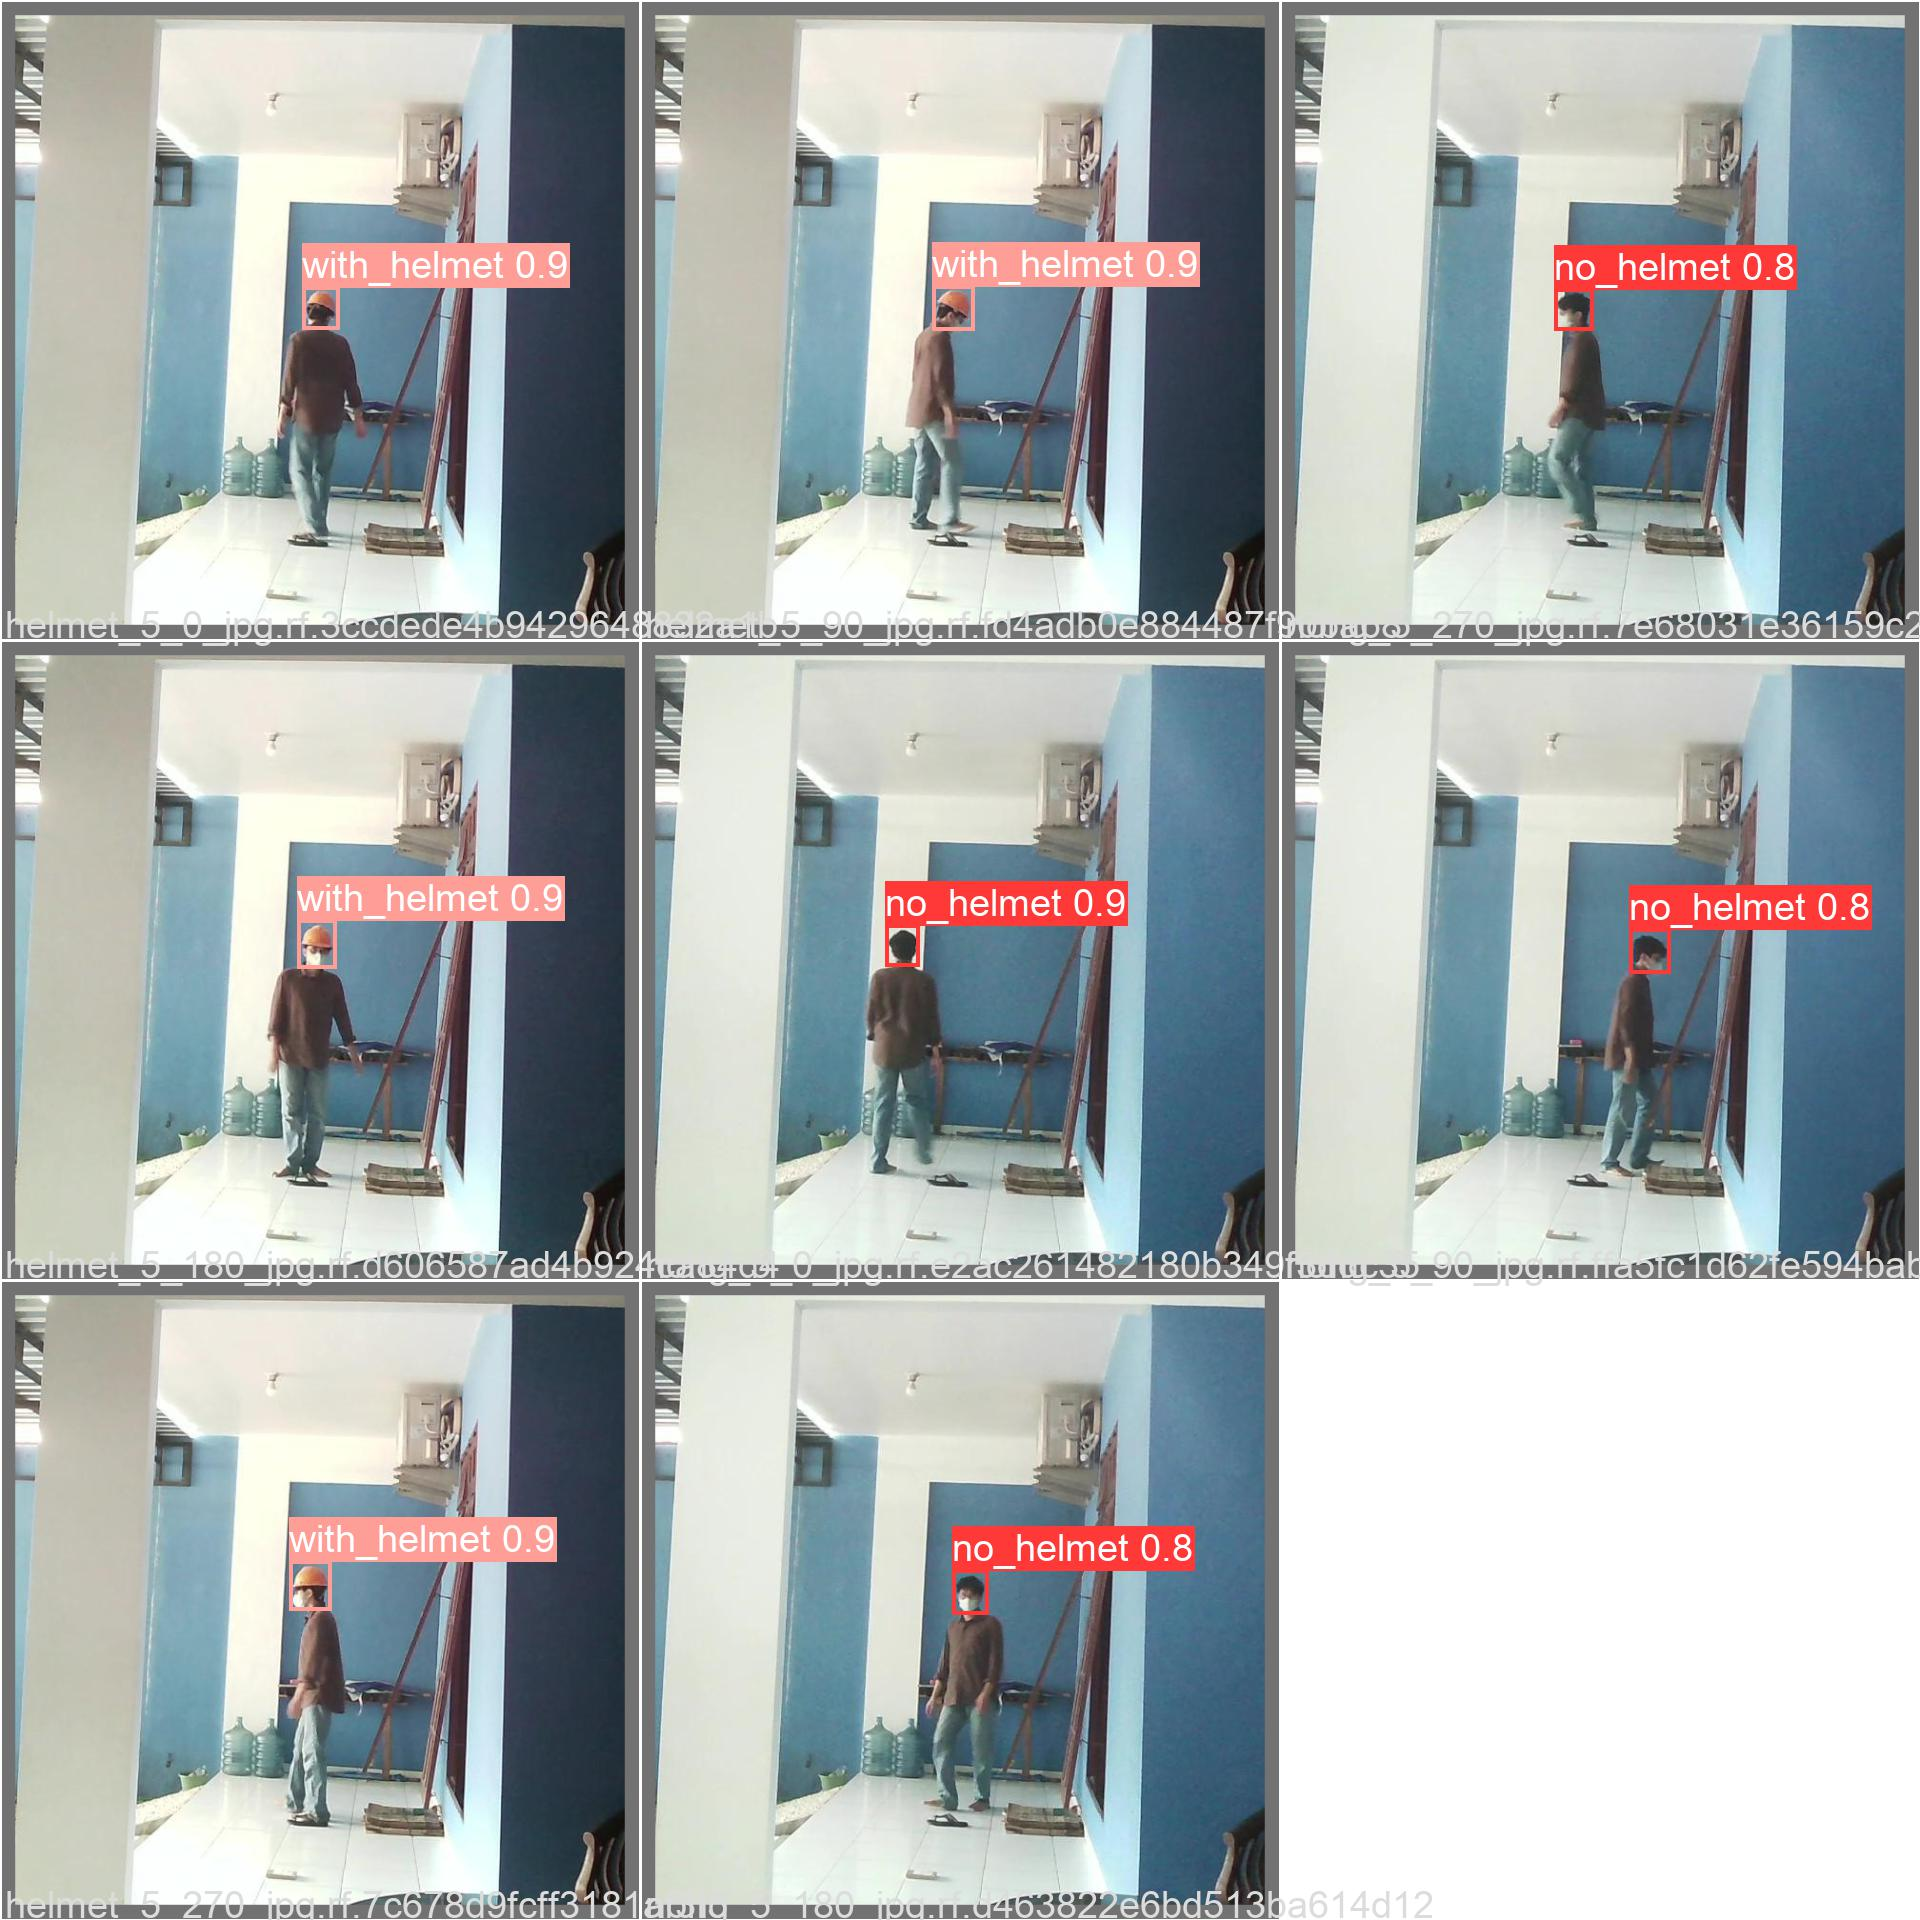
\includegraphics[scale=0.1]{gambar/BerdasarkanJarak/Jarak6_7/val_batch0_pred.jpg}
  \caption{Hasil Prediksi Pada Jarak 6.7 meter}
  % \label{fig:labelbaru}  
\end{figure}

\begin{longtable}{|c|c|c|c|}
  \caption{Konfigurasi Training menggunakan YOLOv5}
  \label{tb:jarak6_7}\\
  \hline
  % \rowcolor[HTML]{C0C0C0}
  \textbf{\emph{Class} }                     & \textbf{\emph{Precision}}  & \textbf{\emph{Recall}} & \textbf{\emph{mAP@.5}}\\
  \hline
  all                                                 & 0.993           & 1        & 0.995         \\
  no\textunderscore helmet                            & 1               & 1        & 0.995          \\
  with\textunderscore helmet                          & 0.986           & 1        & 0.995           \\
  \hline
\end{longtable}


\subsection{Pengujian Pada Jarak 9 Meter}

\begin{figure}[ht]
  \centering
  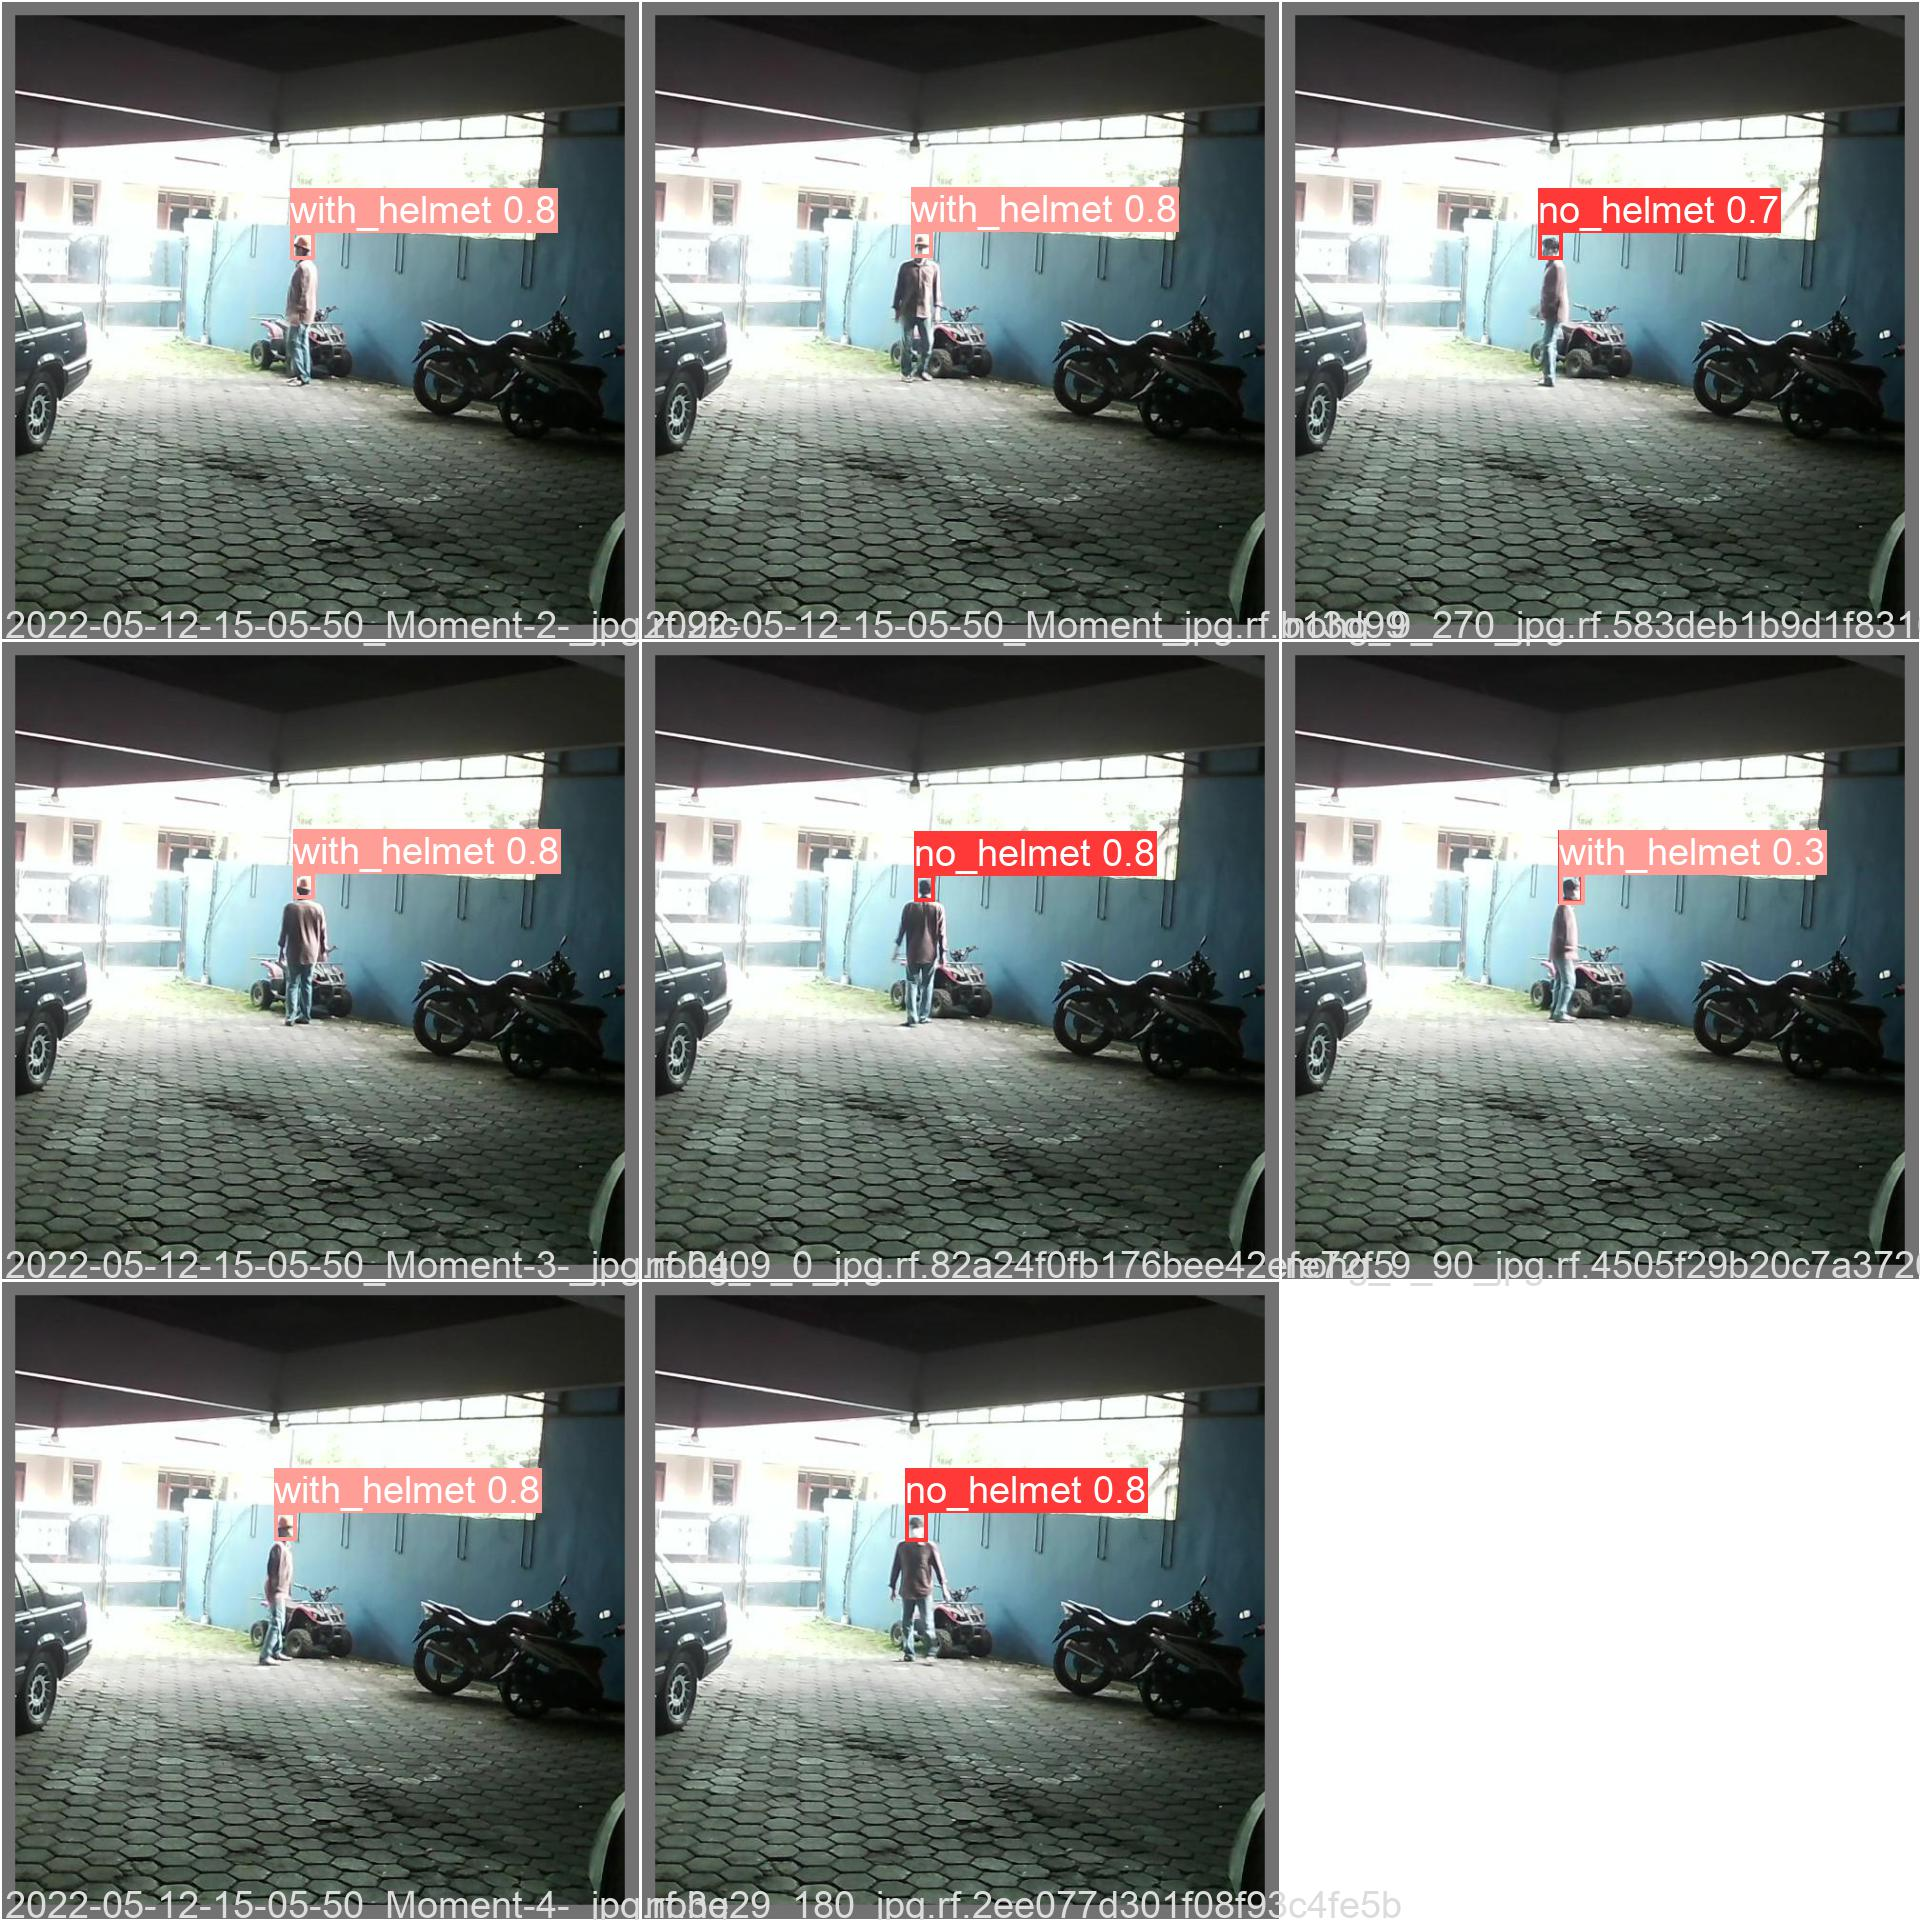
\includegraphics[scale=0.1]{gambar/BerdasarkanJarak/Jarak9/val_batch0_pred.jpg}
  \caption{Hasil Prediksi Pada Jarak 9 meter}
  % \label{fig:labelbaru}  
\end{figure}

\begin{longtable}{|c|c|c|c|}
  \caption{Konfigurasi Training menggunakan YOLOv5}
  \label{tb:jarak9}\\
  \hline
  % \rowcolor[HTML]{C0C0C0}
  \textbf{\emph{Class} }                     & \textbf{\emph{Precision}}  & \textbf{\emph{Recall}} & \textbf{\emph{mAP@.5}}\\
  \hline
  all                                                 & 0.959          & 1        & 0.995         \\
  no\textunderscore helmet                            & 1               & 1        & 0.995          \\
  with\textunderscore helmet                          & 0.918           & 1        & 0.995           \\
  \hline
\end{longtable}